\textbf{10.}

En un estudio realizado en un laboratorio de física educativa, se analizaron los tiempos (en segundos) que tardan varios estudiantes en completar una prueba experimental relacionada con movimiento rectilíneo. Los resultados se organizaron en intervalos y se representaron mediante un histograma para identificar la distribución de los datos. Este tipo de representación es fundamental en estadística, ya que permite visualizar la frecuencia con la que ocurren ciertos valores y detectar tendencias o concentraciones en los datos.

La siguiente gráfica muestra la distribución de frecuencias de los tiempos registrados:

\begin{center}
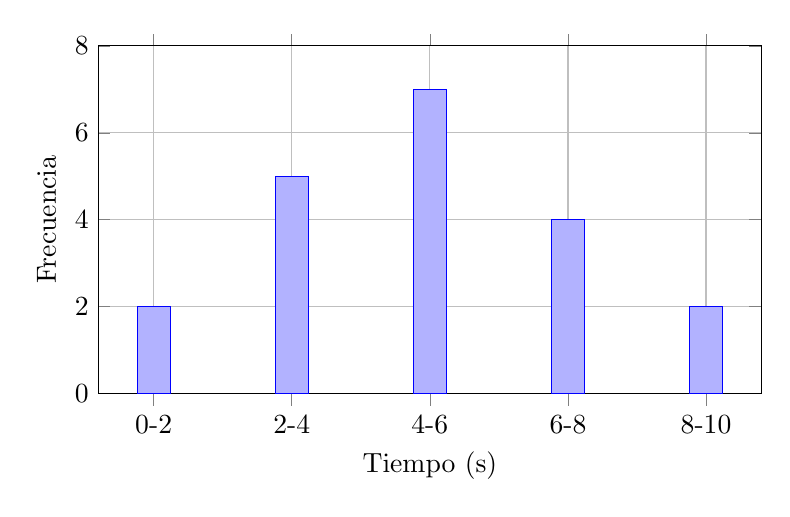
\begin{tikzpicture}
\begin{axis}[
ybar,
bar width=12pt,
width=10cm,
height=6cm,
xlabel={Tiempo (s)},
ylabel={Frecuencia},
xtick=data,
xticklabels={0-2,2-4,4-6,6-8,8-10},
ymin=0,
ymax=8,
grid=both,
]
\addplot coordinates {(1,2) (2,5) (3,7) (4,4) (5,2)};
\end{axis}
\end{tikzpicture}
\end{center}

¿Cuál de las siguientes afirmaciones describe mejor la distribución de los datos?

\begin{multicols}{2}
\begin{enumerate}[label=\alph*), leftmargin=*]
\item La mayor concentración de datos está entre 4 y 6 segundos
\item Los datos están distribuidos uniformemente
\item La menor frecuencia está entre 2 y 4 segundos
\item La mayoría de los estudiantes tardaron más de 8 segundos
\end{enumerate}
\end{multicols}